\chapter{Analysis of Frontal Lobe Fibers}
%make this into a good paper
\section{Schizophrenia}
Schizophrenia is neurological disorder whose characteristic symptoms include hallucinations and disorganized thinking.  Scientists have suggested that the pathology of schizophrenia may involve anatomical abnormalities including abnormal white matter architecture.  Clinical DTI studies have demonstrated differences in diffusion anisotropy within fiber tracts in Schizophrenia patients compared with healthy patients \cite{kubickiBiologPsych03},\cite{kubickiNI05}.

White matter architecture abnormalities related to schizophrenia may include a reduction in the integrity or amount of the myelin, increased disorganization of fibers which constitute certain fiber bundles, or a reduction in the number of fibers comprising a fiber bundle. Myelin, the fatty insulator which surrounds the axons, is believed to be a major barrier to water diffusion.  Degradation of the myelin will permit increased diffusion perpendicular to the orientation of the fibers which can be observed as reduced anisotropy in DTI data.  Also the orientation of axon fibers which comprise a fiber bundle may be less directionally coherent in Schizophrenia.  Since many fibers pass through a single voxel and the resultant diffusion distribution is an average of diffusion of all water molecules that voxel, a voxel containing fibers which are less coherent may have reduced anisotropy.  The fibers bundles may also be less dense in Schizophrenia.  A reduction in axon density would also result in reduced anisotropy water molecules are more free to diffuse perpendicularly to the tracts.  All of these structural deficiencies result in poorer conduction of action potentials between different regions of the brain leading to reduced functional connectivity.

\begin{figure} \label{fig:frontallobefibers}
	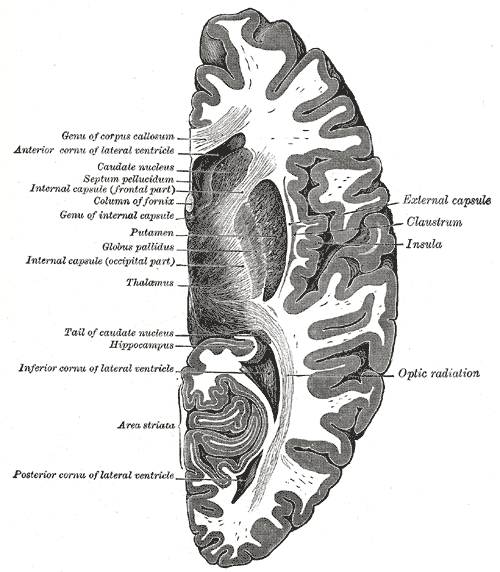
\includegraphics[height=0.5\linewidth]{thalamus}
	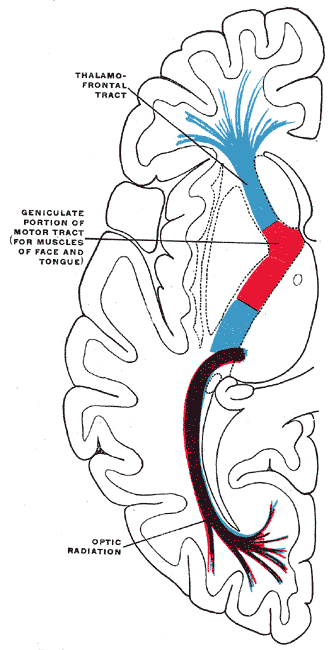
\includegraphics[height=0.5\linewidth]{frontalcortexfibers}
	\caption{The Thalamus, the Internal Capsule and fibers.  We wish to characterize the fibers which originate in the thalamus, pass through the internal capsule and end in the frontal cortex.  This image is from a diagram in Gray's Anatomy}
\end{figure}
The fibers that connect the thalamus and the frontal lobe are believed to be involved in memory formation.  These fibers are depicted in figure \ref{fig:frontallobefibers}.  Since Schizophrenia patients have difficulty forming and organizing memory, deficiencies in these fibers may explain these symptoms.  Additionally these fibers are interesting from a tractography standpoint because there are many other fibers which cross this set of fibers on their way to the frontal cortex.  In these regions of crossing, the diffusion is averaged with the crossing fiber resulting in a diffusion profile with reduced anisotropy.  This is precisely the situation for which stochastic tractography can be useful since streamlining methods would terminate in regions of low anisotropy possibly never reaching the frontal cortex.  In this research, we analyze these fibers in schizophrenia and control groups to determine whether schizophrenia patients exhibit lower tract-averaged fractional anisotropy than the control group.  Additionally, we will compare results obtained using stochastic tractography with previous streamline tractography results.

%show where the labels are using picture
\section{Method}
%talk about the experimental setup
%how was the data obtained
%how many subjects
%the number of gradient directio

%Need to cite how white matter map was obtained


\section{Results}

%convergence results
\begin{figure} \label{fig:facomp}
	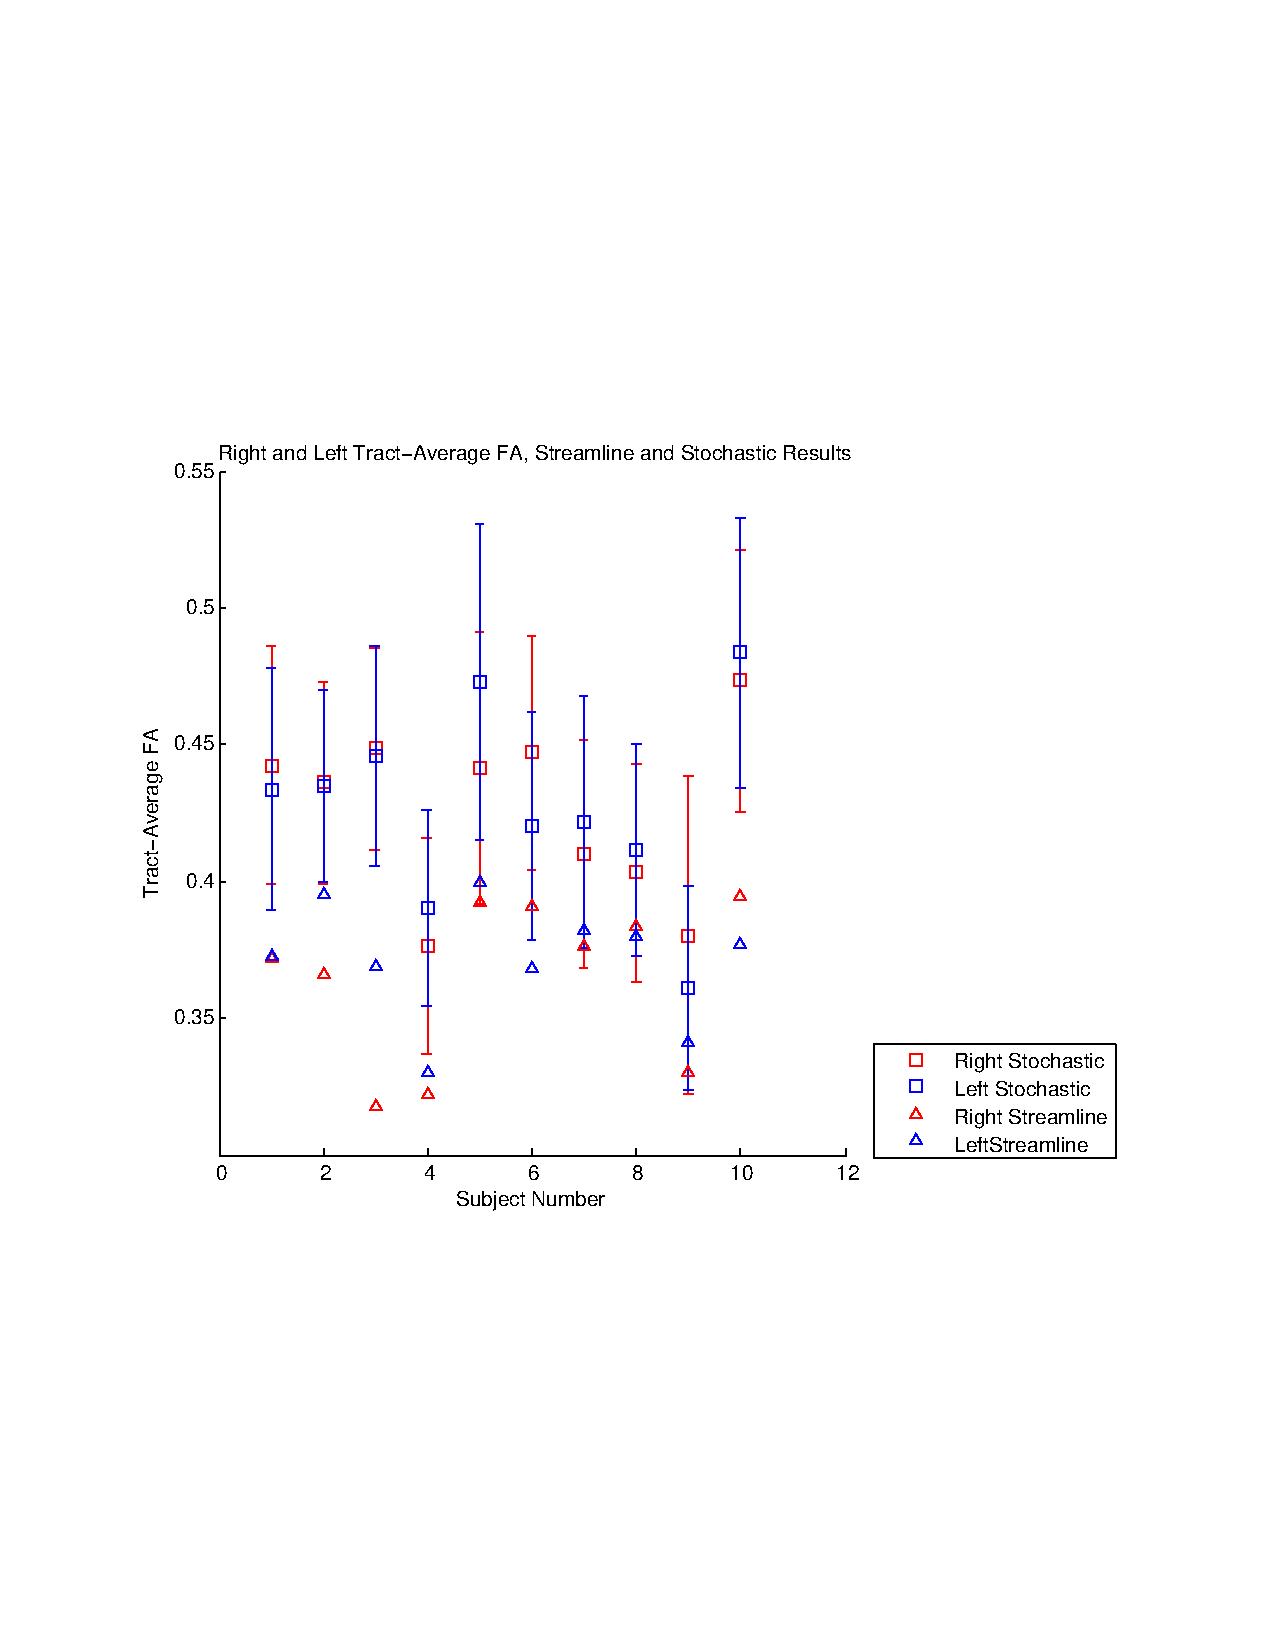
\includegraphics[width=\linewidth]{FAcomp}
	\caption{A graph of tract-averaged FA means for each subject, for the left and right frontal lobe fibers under streamlining tractography and stochastic tractography.  Error bars have a length of two standard deviations.  The FA variance for the tract generated using the streamlining method was not available.  Patients 1-5 are control, patients 6-10 are diagnosed with Schizophrenia. Streamlining results are from research by Gudrun Rosenberger}
\end{figure}

Figure \ref{fig:facomp} graphs the distribution of tract-averaged FA for each patient.  A t-test comparing the mean tract-averaged FA of the schizophrenia group with the control group did not reveal any statistically significant differences.  This was found under both streamlining tractography as well as stochastic tractography.

%T-test

%ANOVA

%\subsection{Convergence of Statistics}
%show graphs of convergence
%Need to determine how to do this
\section{Discussion}
